\chapter{Architecture}

\section{Présentation de l'architecture du projet}
\subsection{Diagramme de flux des données}

\begin{figure}[H]
  \centering
    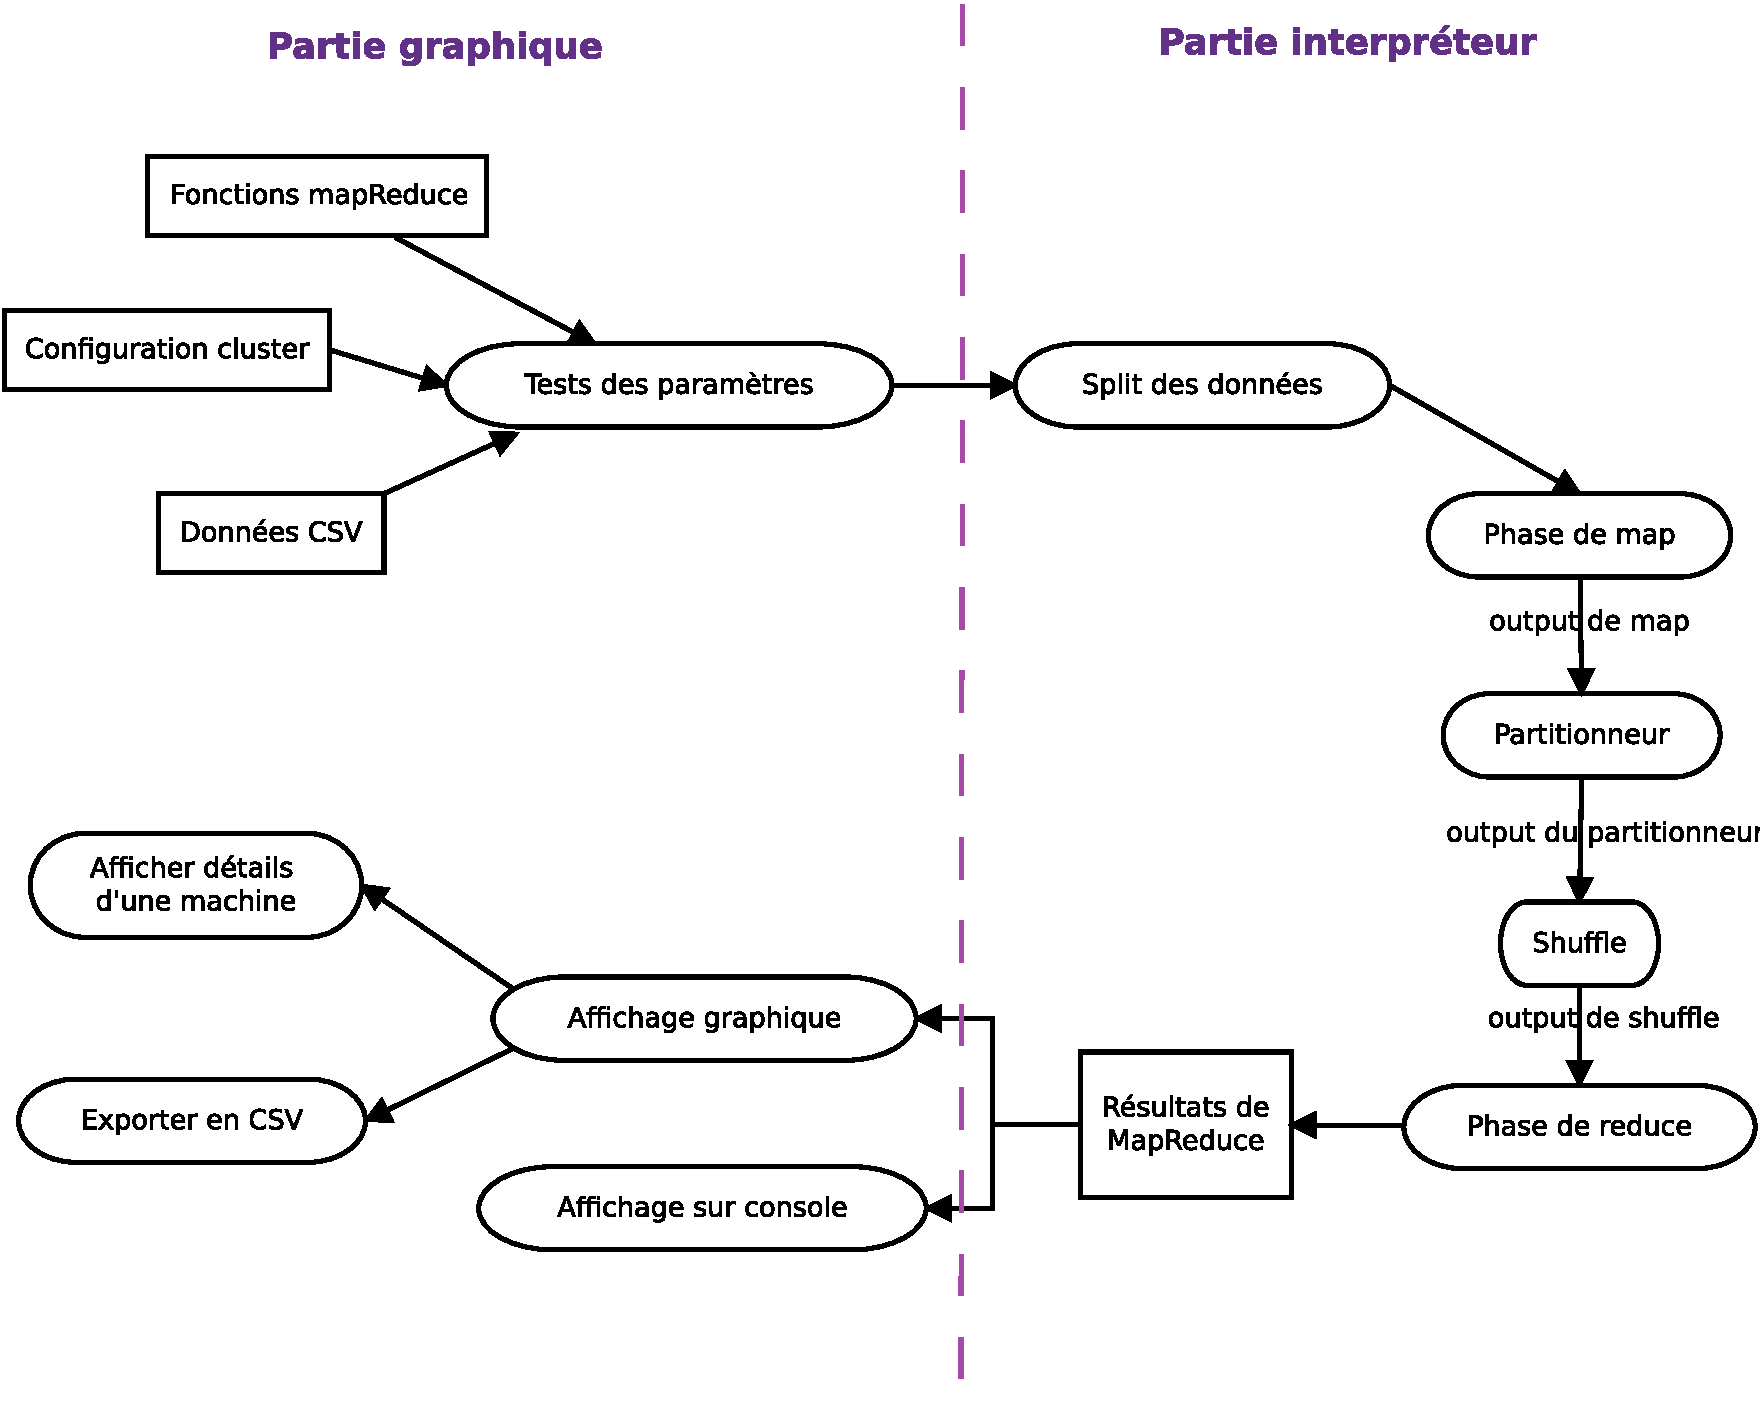
\includegraphics[scale=0.6]{diagram/dfd.pdf}
        \caption{Diagramme de flux des données}
\end{figure}

Ce diagramme de flux des données résume le passage des données en entrée dans une "boite noire" pour ensuite récupérer le résultat final en sortie. Lorsque l'application est lancée, les données sont traitées dans la partie graphique (zone de gauche) puis sont envoyées à la partie interpréteur (zone de droite).

\subsection{Architecture client-lourd | 2-tiers}
Notre projet consiste en un site web qui ne possède pas de base de données. Le serveur ne sert qu'a accéder à son URL\footnote{Uniform Resource Locator} c'est-à-dire qu'il n'est utilisé que pour héberger le contenu du site. Le traitement dans sa totalité se fait du coté du navigateur directement et aucune donnée n'est envoyée/conservée ou reçue d'un serveur.
Ce type d'application correspond donc à l'architecture {\bf Client-lourd}.\\

D'autre part, on remarque que ce projet peut être divisé en deux parties indépendantes, l'une qui va traiter le process de mapReduce, et l'autre qui s'occupe du coté visuel/graphique. On parle ici d'une séparation entre le {\tt traitement} et {\tt l'affichage graphique}.\\
Nous avons donc eu l'idée de suivre l'architecture {\bf 2-couches} pour représenter cette séparation.\\

Ainsi, notre projet reflette une architecture {\bf client-lourd | 2-tiers} combinées pour améliorer l'organisation du travail.

\subsection{Diagrammes de séquence} %a modifier peut etre
\subsubsection{Chargement de la page}

\begin{figure}[H]
  \centering
    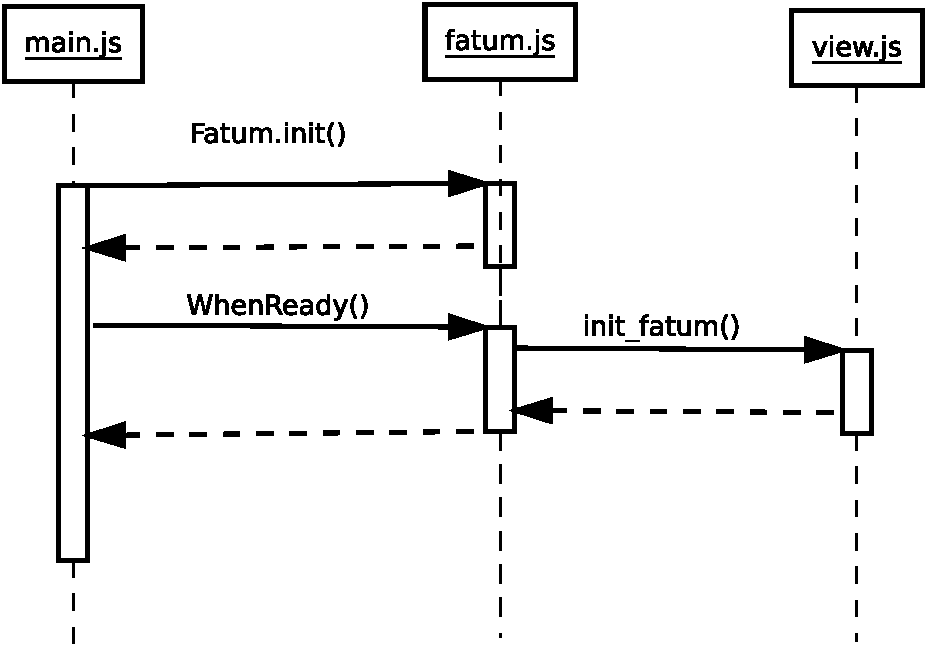
\includegraphics[scale=0.6]{diagram/document.pdf}
        \caption{Chargement de la page}
\end{figure}
Quand l'URL est saisi, la page se met à charger sans aucune intervention de l'utilisateur.
La figure 3.2 représente les différents appels de fonctions lors du chargement de la page. En effet, le chargement se fait par l'initialisation de FATuM appelé dans le fichier {\tt view.js} qui appelle la bibliothèque {\tt fatum.js}.

\subsubsection{Lancement de la simulation}
Lorsque le bouton {\tt Run} est cliqué, une série d'actions se produit.
D'abord, le cluster est affiché (sans les connections). Ensuite, le traitement de mapReduce est effectué. Enfin, les connections entre les slots sont affichées.\\
Ces actions sont représentées par trois parties dans les figures 3.3, 3.4 et 3.5.
\begin{figure}[H]
  \centering
    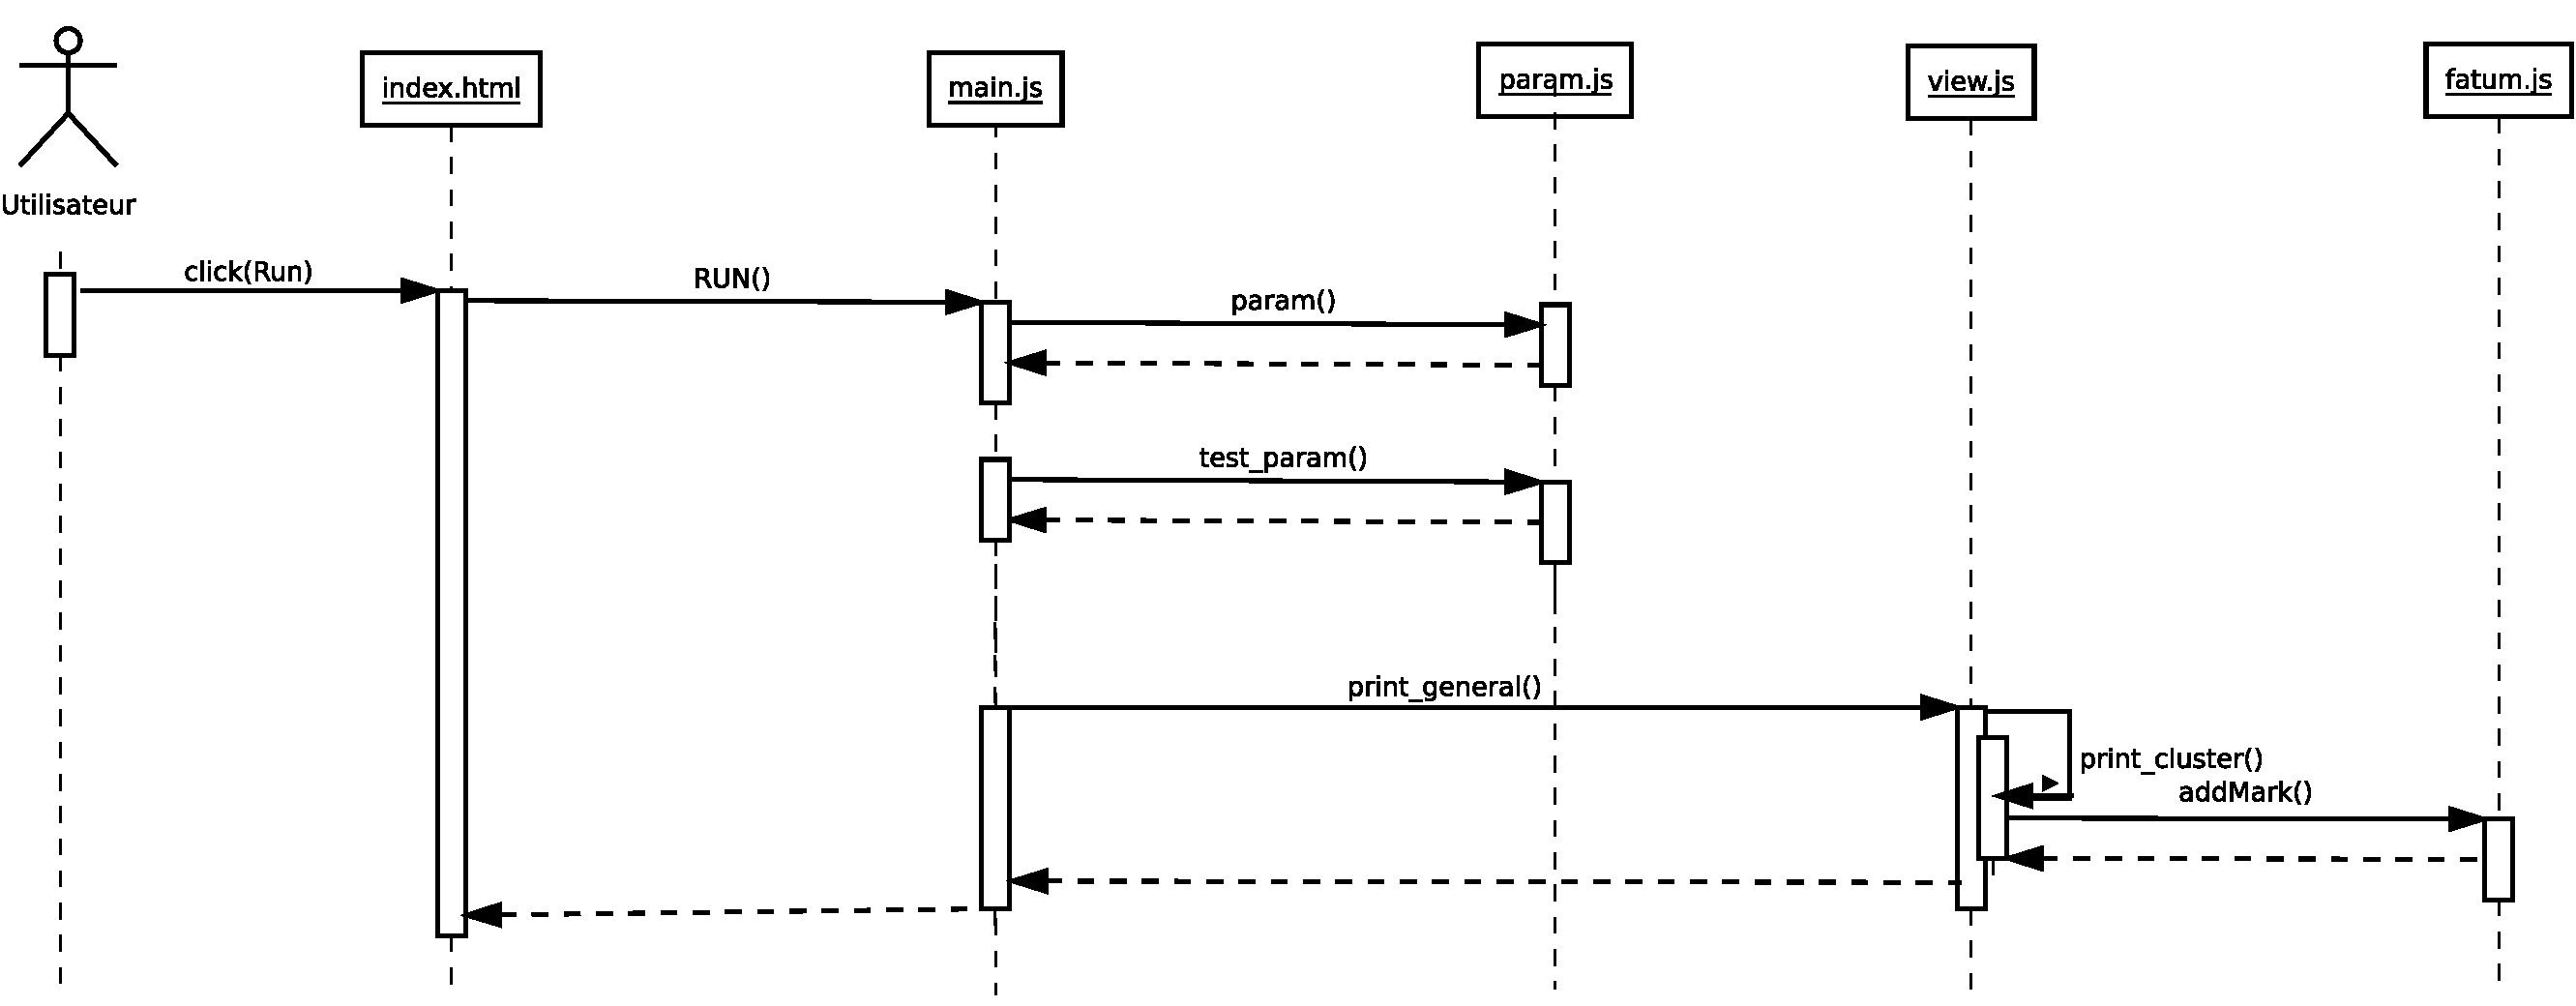
\includegraphics[angle=90,scale=0.5]{diagram/diag_seq_init.pdf}
        \caption{Lancement du bouton RUN}
\end{figure}
Lors de l'affichage du cluster, les données fournies par l'utilisateur doivent respecter certaines conditions imposées par la fonction {\tt Test\_param} (par exemple entrer un nombre supérieur à 1 pour le nombre de PC). Une fois les conditions d'utilisation passées, on appelle la bibliothèque FATuM pour afficher les différents slots du cluster de Map et de Reduce ainsi que les numéros des PC (affichage sans les connections entre les slots).

\begin{figure}[H]
  \centering
    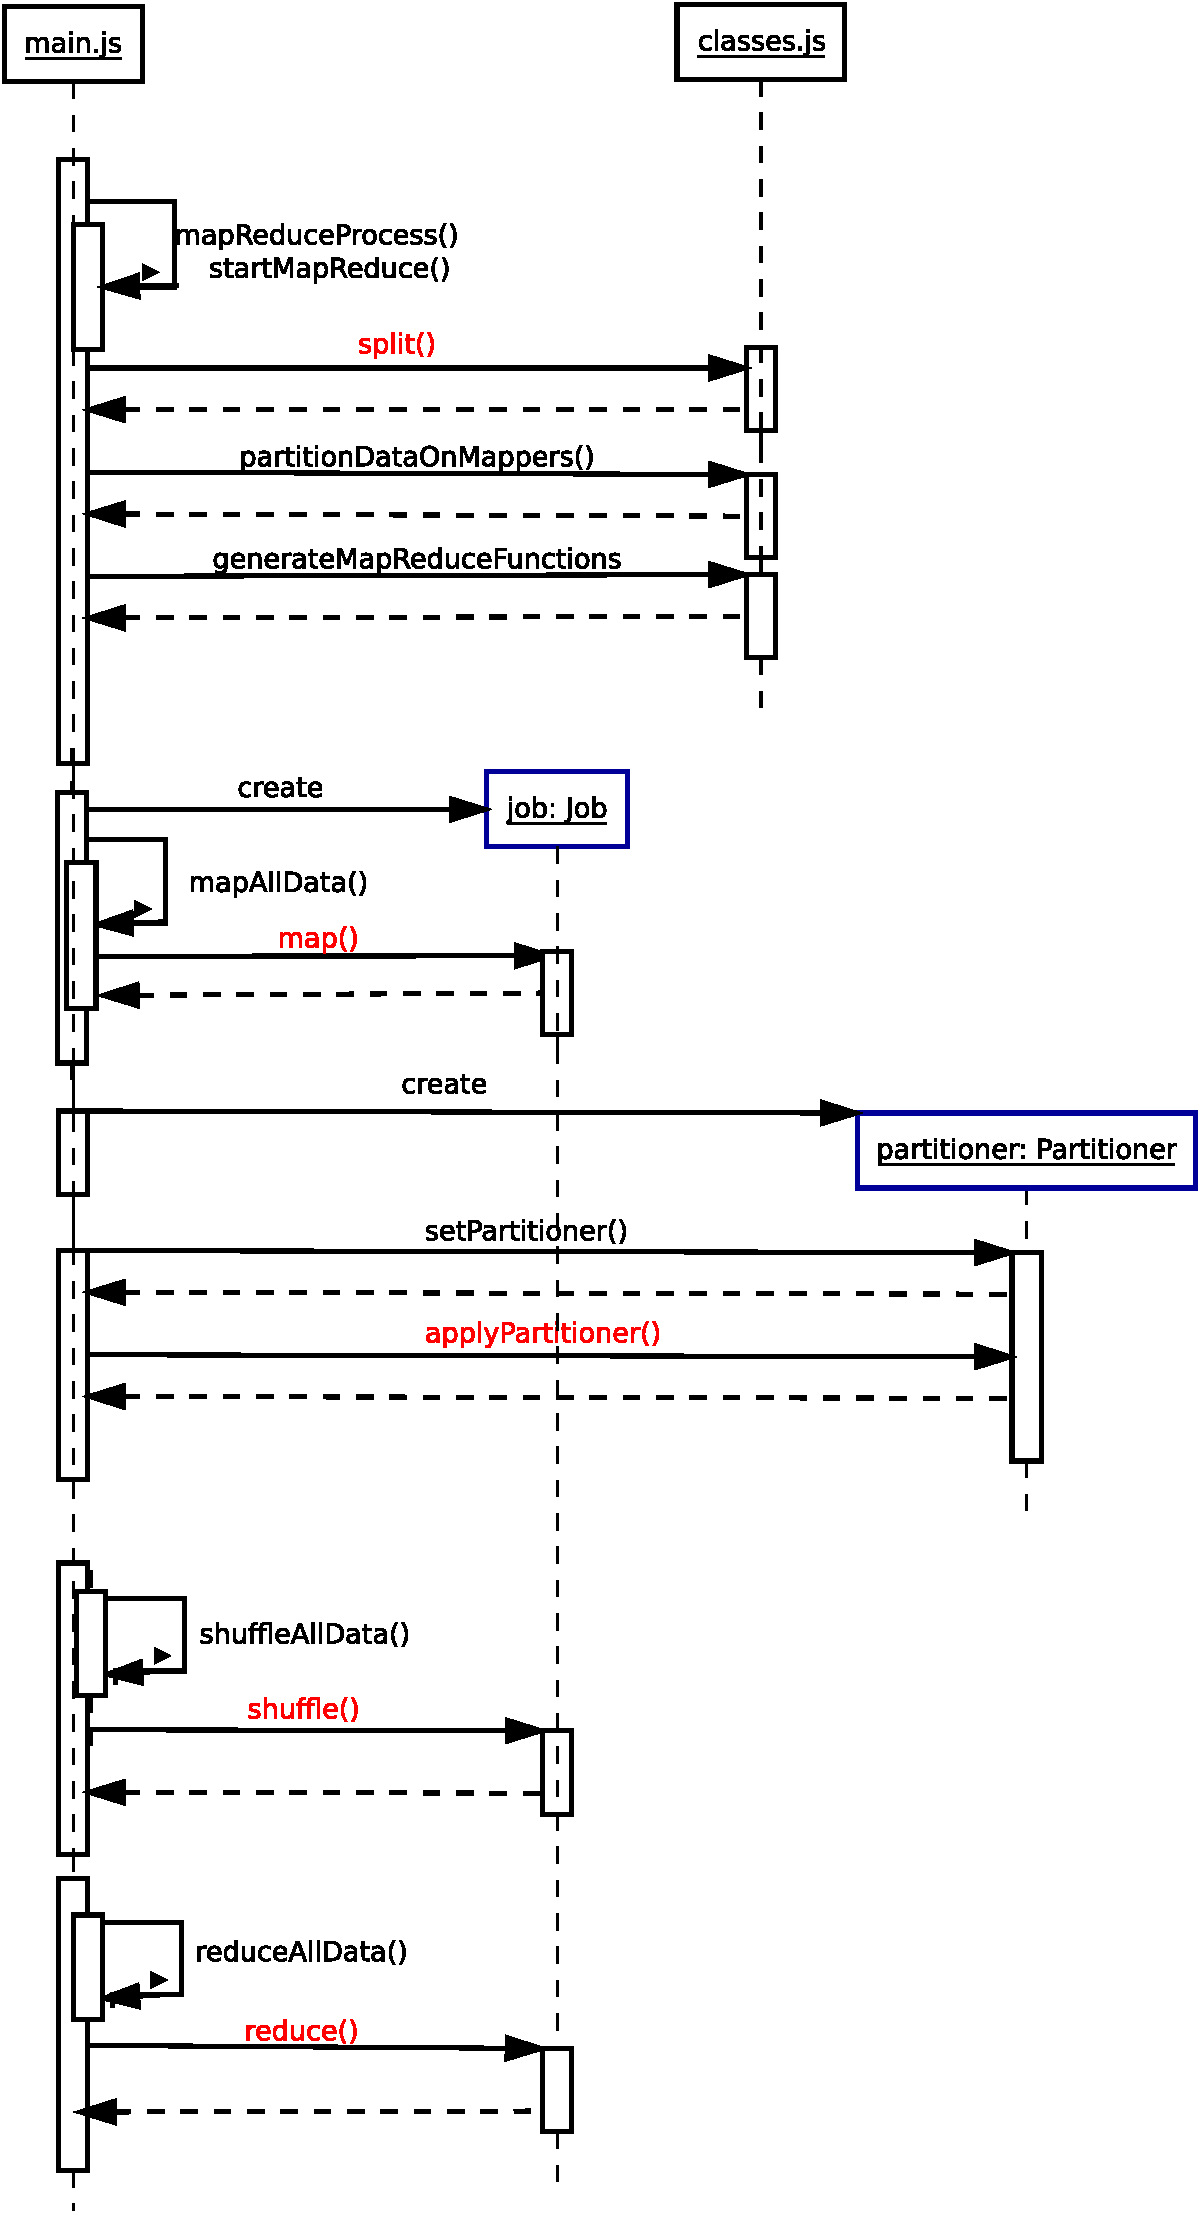
\includegraphics[scale=0.6]{diagram/diag_seq_mapReduce.pdf}
        \caption{Process de MapReduce}
\end{figure}

Une fois les éléments du cluster de la simulation affichés, le traitement des données s'effectue. Après chaque traitement, on effectue un lien entre chaque slot du cluster pour indiquer le transfert des données au sein de ce dernier représenté par des flèches provenant de FATuM.

\begin{figure}[H]
  \centering
    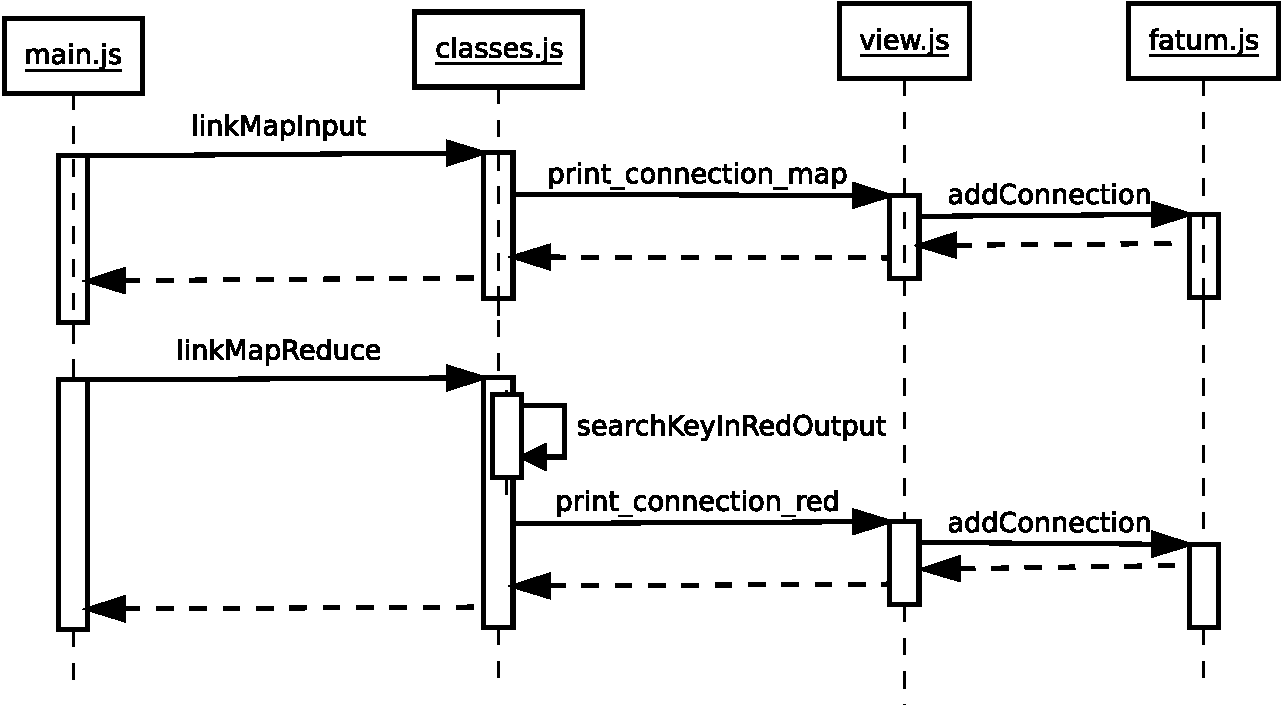
\includegraphics[scale=0.6]{diagram/print_connection.pdf}
        \caption{Affichage des connections}
\end{figure}

\subsubsection{Récupérer les données traitées}
\begin{figure}[H]
  \centering
    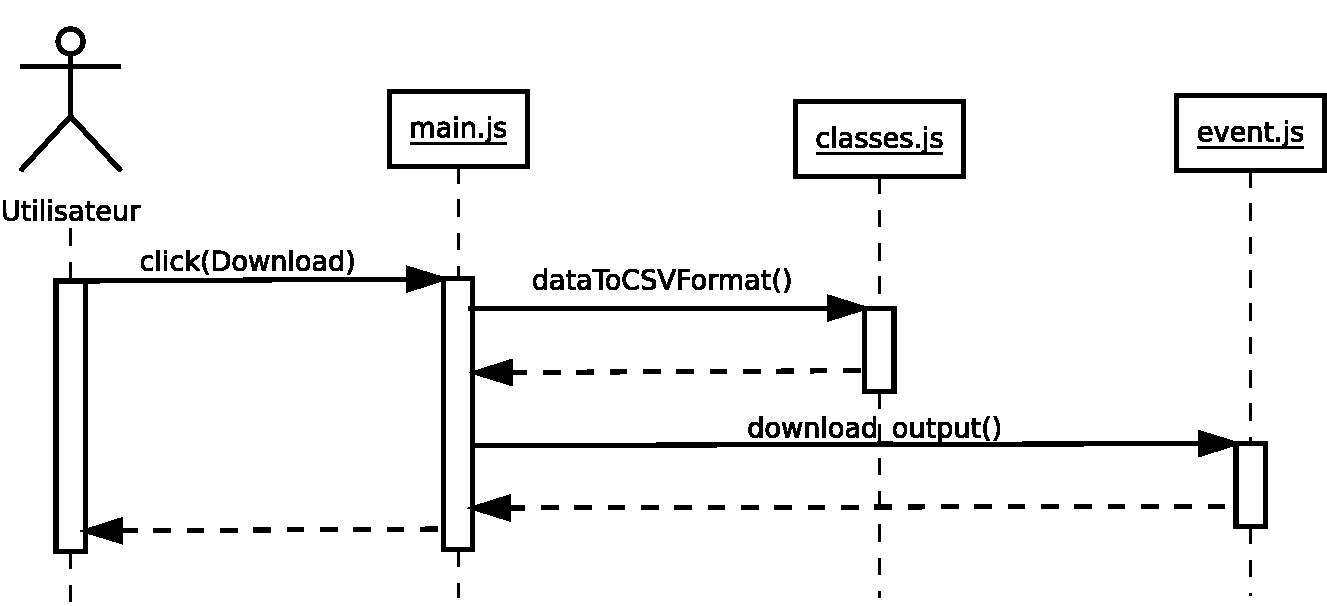
\includegraphics[scale=0.6]{diagram/download.pdf}
        \caption{Lancement du bouton Download}
\end{figure}
Une fois la simulation et le traitement des données effectué. L'utilisateur peut récupérer ces données transformer par ses fonctions mapReduce en les téléchargeant dans un format CSV.
%\section{Outils utilisés}

